\chapter{Crescimento de domínios}
 \label{cap.Crescimento}


\section{Introdução}

Encontramos na natureza diversos sistemas que podem existir em fases de equilíbrio claramente distintas quanto a um critério de ordem ou simetria. Um típico exemplo é o de sistemas que apresentam ferromagnetismo, fenômeno exibido por metais como ferro, níquel, cobalto, e suas ligas, que apresentam as fases paramagnética e ferromagnética. Na fase paramagnética, acima de uma temperatura crítica denominada temperatura de Curie, o sistema possui magnetização total nula na ausência de campo magnético externo. Já na fase ferromagnética, abaixo da temperatura de Curie, na ausência de campo magnético externo, o sistema apresenta uma magnetização total não-nula em uma particular direção, denominada magnetização espontânea. Na fase ferromagnética, portanto, o sistema tem uma determinada direção privilegiada, dada pela direção da magnetização espontânea, possuindo assim um grau de simetria menor do que na fase paramagnética.

A base do fenômeno ferromagnético está no alinhamento dos spins eletrônicos (que estão associados a um momento magnético), devido fundamentalmente à interação de troca entre os elétrons. Na fase paramagnética, as flutuações térmicas são mais importantes que as interações entre spins, fazendo com que os spins apresentem apenas correlações de curto alcance, levando a um desordenamento global do sistema, e por consequência a uma magnetização total nula. Na fase ferromagnética, no entanto, as forças de interação tornam-se mais importantes que as flutuações térmicas, favorecendo um alinhamento dos spins em uma particular direção e levando a uma magnetização total não-nula. A particular direção de alinhamento dos spins é determinada por flutuações térmicas existentes durante a transição entre as fases, podendo ainda estar sujeita a restrições impostas pela estrutura cristalina do material. Diz-se que ao sofrer uma transição da fase paramagnética para a fase ferromagnética o sistema passa por uma quebra espontânea de simetria.

Após uma queda brusca de temperatura, de um valor acima da temperatura de Curie para uma temperatura abaixo desta (\textit{quench}), o sistema não chega instantaneamente a um estado de equilíbrio com um alinhamento global dos spins, mas é levado para fora do equilíbrio, evoluindo em direção ao mesmo de acordo com uma dinâmica lenta, que apresenta diferentes domínios magnéticos competindo entre si, cada um se apresentando como uma região com uma particular direção de magnetização. Durante a evolução do sistema, após o \textit{quench}, verifica-se a existência de uma dinâmica de separação de fases, ou de crescimento dos domínios magnéticos (\textit{coarsening}).


\section{O modelo de Ising}

O modelo de Ising é um dos modelos mais simples e mais amplamente estudados da mecânica estatística. Ele foi proposto como uma forma de tentar reproduzir de forma simplificada o comportamento de um sistema ferromagnético. O modelo define um conjunto de spins que podem, individualmente, assumir os valores -1 ou +1, dispostos sobre os sítios de uma rede com determinada geometria, onde cada spin interage com seus vizinhos e possivelmente com um campo magnético externo.

Introduzido na tese de doutorado de Ernest Ising, em 1920, o modelo teve sua resolução exata em uma dimensão apresentada no trabalho, onde foi constatada a inexistência de transições de fases em uma dimensão.

Em 1944, Lars Onsager \cite{Onsager} obteve a solução exata para o modelo na rede bidimensional quadrada a campo externo nulo, onde foi comprovada a existência de transição de fase. Para campo externo nulo, o modelo pode ser descrito pelo hamiltoniano:
\begin{equation}
  {\cal H} = -J \sum_{\langle i,j \rangle} S_i S_j,
\end{equation}
onde o somatório é computado apenas sobre primeiros-vizinhos e $J$ é uma constante de acoplamento que determina o tipo e a magnitude da interação entre os spins. Para $J>0$ temos uma interação ferromagnética, enquanto que para $J<0$ temos uma interação antiferromagnética.

A transição entre as fases para e ferromagnética é contínua e ocorre na temperatura crítica $T_c = 1/\ln(1+\sqrt{2})$, em unidades de $J/k_B$.


\section{O modelo de Potts}

Introduzido em 1951, na tese de doutorado de Renfrey Potts, o modelo de Potts pode ser considerado como uma generalização do modelo de Ising para o caso de estados fundamentais com múltipla degenerescência~\cite{Wu}. Assim como o modelo de Ising, o modelo de Potts define um conjunto de spins que podem assumir valores discretos, normalmente dispostos sobre os sítios de uma rede com determinada geometria, com interação entre spins vizinhos, e possivelmente com um campo magnético externo. Entretanto, no modelo de Potts, cada spin pode individualmente assumir $q$ valores distintos (e.g., $0$ a $q-1$). Para campo externo nulo, o modelo pode ser descrito pelo hamiltoniano:
\begin{equation}
 {\cal H} = -J \sum_{\langle i,j \rangle} \delta_{S_i S_j},
\end{equation} 
onde o somatório é computado apenas sobre primeiros-vizinhos e $\delta$ é a função delta de Kronecker.

Para $q=2$ o modelo é equivalente ao modelo de Ising, a menos de uma constante, permanecendo válida a solução de Onsager em duas dimensões. Embora a solução exata para o modelo em duas dimensões, em uma rede quadrada, seja conhecida apenas para $q=2$, grande parte de suas propriedades são conhecidas. A sua temperatura crítica é $T_c(q) = 1/\ln(1+\sqrt{q})$, em unidades de $J/k_B$. Para $q \le 4$ a transição é contínua, enquanto que para $q>4$ é de primeira ordem. Na figura \ref{fig.MagPotts} pode-se observar a variação da magnetização em função da temperatura para o Modelo de Potts, para diversos valores de $q$. Embora os efeitos de tamanho finito sejam aparentes, pode-se perceber claramente a descontinuidade para valores grandes de $q$.

\begin{figure}
 \centering
 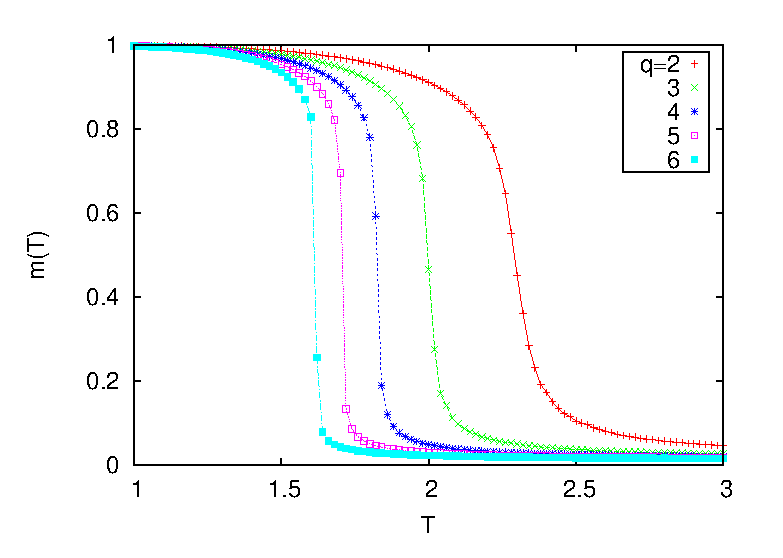
\includegraphics[width=14cm]{img/MagPotts.eps}
 \caption{Magnetização para o modelo de Potts, com $q=2, 3, 4, 5, 6$. Nota-se a presença de duas fases: uma desordenada, onde a magnetização é quase nula (fase paramagnética) e outra ordenada, onde a magnetização tem um valor próximo a $1$ (fase ferromagnética). Os resultados foram obtidos através de uma simulação usando o algoritmo do banho térmico, para uma rede bidimensional quadrada com dimensão linear $L=60$.}
\label{fig.MagPotts}
\end{figure}


\section{Domínios geométricos e \textit{hulls}}

Dois conceitos utilizados no estudo da morfologia de modelos de spins são os de domínios geométricos e \textit{hulls}, exemplificados na figura~\ref{fig.DomainsHulls}. Um domínio geométrico é definido como um agrupamento de spins com a mesma orientação, tal que quaisquer dois spins pertencentes ao mesmo podem ser conectados por um caminho composto de outros spins com a mesma orientação, e que pode ser percorrido com passos entre primeiros vizinhos. A área do domínio corresponde à superfície desse agrupamento, que no caso de spins discretos corresponde ao número de spins contidos no agrupamento. Domínios geométricos podem conter e estar contidos em outros domínios geométricos. Um \textit{hull} é definido como o contorno externo de um domínio geométrico, e sua área corresponde à área desse domínio geométrico, mais as áreas de todos os outros domínios geométricos por ele englobados.

A justificativa para a introdução do conceito de \textit{hull}, que pode parecer menos natural que o conceito de domínio geométrico, reside no fato que a determinação das áreas dos \textit{hulls} é um problema mais facilmente tratável por métodos analíticos, por essas áreas dependerem de uma única interface, facilitando assim a obtenção de expressões exatas.

Embora outros tipos de domínios sejam também utilizados em estudos relacionados a modelos de spins, como domínios de Fortuin-Kasteleyn~\cite{FortuinKasteleyn}, o presente trabalho se limita a estudar propriedades associadas aos domínios geométricos (podendo aqui ser chamados simplesmente de domínios).

\begin{figure}
 \centering
 \includegraphics[width=6cm]{img/DomainsHulls.pdf}
 \caption{Exemplo de configuração com quatro \textit{hulls} e quatro domínios geométricos circulares. O \textit{hull} mais externo, de raio $R_1$, contém dois \textit{hulls} de primeira geração, de raios $R_2$ e $R_3$, e um \textit{hull} de segunda geração, de raio $R_4$. O \textit{hull} de raio $R_1$ engloba uma área de $\pi R_1^2$, enquanto que o domínio geométrico de raio $R_1$ tem uma área de $\pi(R_1^2-R_2^2-R_3^2)$~\cite{PREJeferson}.}
\label{fig.DomainsHulls}
\end{figure}


\section{Escalamento dinâmico}

Observa-se em diversos sistemas que apresentam uma dinâmica de crescimento de domínios, ao evoluírem fora do equilíbrio, tanto experimentalmente como em simulações numéricas, que as estruturas formadas pelos domínios são estatisticamente similares em diferentes tempos, a menos de um fator de escala global. Essa observação levou à formulação da hipótese fenomenológica do escalamento dinâmico, que afirma que existe no sistema um único comprimento característico $R(t)$, que cresce com o tempo, de forma que o padrão das estruturas é estatisticamente independente do tempo quando todos os comprimentos são especificados em unidades de $R(t)$~\cite{ReviewBray}. Lifshitz e Slyozov~\cite{Lifshitz1961,Lifshitz1962} determinaram que em sistemas nos quais o parâmetro de ordem não é conservado, o que inclui os modelos de Ising e de Potts (para qualquer valor de $q$) conforme aqui apresentados, o comprimento característico $R(t)$ é bem descrito por:
\begin{equation}
 R(t) \sim t^{1/2}. 
\end{equation}


\section{Dinâmica de crescimento}

Observa-se no modelo de Ising, após um \textit{quench} através da temperatura crítica, uma dinâmica de crescimento de domínios, conforme se pode observar na figura \ref{fig.IsingSnap}.

\begin{figure}[h!]
 \setlength\fboxsep{0pt}
 \setlength\fboxrule{0.5pt}
 \centering
 \fbox{\includegraphics[width=35mm]{img/Ising_scr1.png}}
 \fbox{\includegraphics[width=35mm]{img/Ising_scr2.png}}
 \fbox{\includegraphics[width=35mm]{img/Ising_scr3.png}}
 \fbox{\includegraphics[width=35mm]{img/Ising_scr4.png}} \\
 (a) \hspace{30mm} (b) \hspace{30mm} (c) \hspace{30mm} (d) \vspace{3mm} \\
 \caption{Sequência mostrando a evolução de uma simulação de Monte Carlo do modelo de Ising, após um \textit{quench} da temperatura infinita para a temperatura zero. Os respectivos tempos são $t=2,8,32,256$ passos de Monte Carlo (MCs). Pontos pretos e brancos representam spins com valores $-1$ e $+1$. Para $t \rightarrow \infty$ o sistema atinge ou um estado ordenado, ou um estado formado por listras de spins com a mesma orientação~\cite{BlanchardPicco}.}
 \label{fig.IsingSnap}
\end{figure}

Em 1979, Allen e Cahn~\cite{AllenCahn} verificaram que a velocidade de um elemento de área de uma interface entre dois domínios, para sistemas com parâmetro de ordem não conservado, está relacionada à curvatura local dessa interface, obtendo a relação, válida para qualquer dimensão:
\begin{equation}
 \label{eq.AllenCahn}
 v=-\frac{\lambda}{2\pi} \kappa,
\end{equation}
onde $\lambda$ é um parâmetro dependente da temperatura, com dimensões de constante de difusão, $\kappa$ a curvatura local, e $v$ a velocidade do elemento de área da interface, normal a cada ponto da mesma, com sentido na direção que determina a redução da curvatura.

Podemos expressar a variação da área englobada por um \textit{hull} através de uma integral de caminho, sobre o \textit{hull}, da velocidade de um elemento diferencial do mesmo:
\begin{equation}
 \label{eq.DaDtq2}
 \frac{dA_h}{dt} = \oint v dl = -\frac{\lambda_h}{2\pi} \oint \kappa dl = -\lambda_h,
\end{equation}
onde\footnote{Utilizamos aqui $\lambda_h$ para denotar o parâmetro associado com a variação de áreas englobadas por \textit{hulls}, enquanto que para o caso de domínios geométricos, o parâmetro será denotado por $\lambda_d$.} a última igualdade é obtida a partir do teorema de Gauss-Bonnet~\cite{PRLJeferson}. Integrando a Eq.~(\ref{eq.DaDtq2}) no tempo, chega-se a:
\begin{equation}
 \label{eq.Area}
 A_h(t) = A_h(0) - \lambda_h t.
\end{equation}
Ou seja, independentemente de suas áreas, todos os \textit{hulls} diminuem com a mesma taxa. Definindo $n_h(A,t)$ como a distribuição das áreas dos \textit{hulls}, tal que $n_h(A, t)dA$ é o número de \textit{hulls} com áreas entre $A$ e $A+dA$ no tempo $t$, usando a Eq.~(\ref{eq.Area}), temos:
\begin{equation}
 \label{eq.DistHulls}
 n_h(A,t) = n_h(A+\lambda_h t,0).
\end{equation}

Observa-se que, conhecida a distribuição inicial das áreas dos \textit{hulls}, pode-se determinar a distribuição em qualquer tempo subsequente, e que a distribuição mantém a sua forma durante a evolução temporal, apenas se deslocando na direção de áreas menores.


\section{Distribuições de áreas de \textit{hulls} para $q=2$}

A forma da distribuição das áreas dos \textit{hulls} para o modelo com dois estados (Ising, ou, equivalentemente, Potts com $q=2$), para a condição de equilíbrio na temperatura crítica, foi determinada por Cardy e Ziff em 2003~\cite{Cardy2003}. A expressão obtida para esse caso equivale a:
\begin{equation}
 \label{eq.hq2t0Tc}
 n_h(A,0) \sim \frac{c_h}{A^2}, \qquad T_0 = T_c,
\end{equation}
onde $c_h = 1/(8\pi\sqrt{3})$ é uma constante universal. A expressão é válida para $A_0 \ll A \ll L^2$, sendo $A_0$ uma área microscópica, da ordem de grandeza da área ocupada por uma partícula, e $L^2$ o tamanho do sistema.

Cardy e Ziff determinaram ainda a forma da distribuição das áreas dos \textit{hulls} para um modelo de percolação aleatória na densidade crítica. Um modelo de percolação aleatória pode ser definido sobre uma rede com determinada geometria, onde cada sítio pode estar ocupado por uma partícula ou vazio, com uma distribuição aleatória das partículas, sendo que sítios ocupados adjacentes (primeiros vizinhos) são considerados como pertencentes a um mesmo agrupamento, \textit{cluster} ou domínio, sendo os \textit{hulls} definidos da mesma forma que para os modelos de spins. Para uma densidade de ocupação de sítios $\rho$ maior que determinada densidade crítica $\rho_c$, surge no sistema um domínio de dimensões macroscópicas (ou percolante), que ocupa uma fração finita do tamanho total do sistema (sendo infinito, para um sistema infinito)~\cite{Stauffer}. A expressão encontrada para a distribuição das áreas dos \textit{hulls} para esse caso foi a mesma encontrada para o modelo de dois estados para a condição de equilíbrio na temperatura crítica, ou seja:
\begin{equation}
 \label{eq.nrandperc}
 n_p(A) \sim \frac{c_h}{A^2}, \qquad \rho = \rho_c.
\end{equation}

Embora a distribuição das áreas dos \textit{hulls} para o modelo com dois estados, para a temperatura infinita, não seja conhecida exatamente, Arenzon \textit{et al}~\cite{PRLJeferson} mostraram, através de simulações, que o estado do modelo nessas condições se aproxima rapidamente do estado do modelo de percolação aleatória na densidade crítica. Esse comportamento pode ser explicado por termos, quando $T \rightarrow \infty$, uma igual probabilidade de encontrar os spins em cada um dos dois possíveis estados. Podemos assim estabelecer uma correspondência entre os dois estados possíveis do spin e os estados possíveis de um sítio no modelo de percolação aleatória (ocupado ou vazio), e dizer que temos um caso equivalente ao do modelo de percolação aleatória com uma densidade de ocupação $\rho = 1/2$, que se aproxima do valor da densidade crítica $\rho_c$. Assim, temos:
\begin{equation}
 \label{eq.hq2t0Tinf}
 n_h(A,0) = 2 n_p(A) \sim \frac{2c_h}{A^2}, \qquad T_0 \rightarrow \infty,
\end{equation}
onde o fator 2 se justifica pela existência de dois tipos de domínios, correspondentes aos dois estados do modelo, enquanto que o resultado obtido para o modelo de percolação aleatória considera apenas domínios de sítios ocupados (e não domínios de sítios vazios)~\cite{PRLJeferson}.

Considerando as Eq.~(\ref{eq.hq2t0Tc}) e (\ref{eq.hq2t0Tinf}) como condições iniciais da Eq.~(\ref{eq.DistHulls}), chega-se a:
\begin{equation}
 \label{eq.hq2tTinf}
 n_h(A,t) = \frac{2c_h}{\left(A + \lambda_h t \right)^2}, \qquad T_0 \rightarrow \infty,
\end{equation}
\begin{equation}
 \label{eq.hq2tTc}
 n_h(A,t) = \frac{c_h}{\left(A + \lambda_h t\right)^2}, \qquad T_0 = T_c.
\end{equation}

As distribuições dadas pelas Eq.~(\ref{eq.hq2tTinf}) e (\ref{eq.hq2tTc}) correspondem a sistemas com áreas características proporcionais a $t$, ou comprimentos característicos proporcionais a $t^{1/2}$, validando o resultado previsto pela hipótese de escalamento dinâmico.


\section{Distribuições de áreas de domínios geométricos para $q=2$}
\label{sec.DistAreasDomGeo}

Arenzon \textit{et al}~\cite{PRLJeferson,PREJeferson} mostraram que as formas das distribuições de áreas de domínios geométricos são similares às obtidas para as áreas dos \textit{hulls}, sendo descritas pelas expressões:
\begin{equation}
 \label{eq.dq2tTinf}
 n_d(A,t) = \frac{2c_d}{\left(A + \lambda_d t \right)^{\tau^\prime}}, \qquad T_0 \rightarrow \infty,
\end{equation}
\begin{equation}
 \label{eq.dq2tTc}
 n_d(A,t) = \frac{c_d}{\left(A + \lambda_d t\right)^\tau}, \qquad T_0 = T_c,
\end{equation}
onde $\tau^\prime = 187/91 \approx 2.055$, $\tau = 379/187 \approx 2.027$, e $c_d \approx c_h$. Na figura \ref{fig.areas_q2_L256} pode-se observar uma comparação entre resultados descritos pelas Eq.~(\ref{eq.dq2tTinf}) e (\ref{eq.dq2tTc}), e obtidos através de simulações numéricas baseadas no método de Monte Carlo.

\begin{figure}[h!]
 \centering
 \includegraphics[width=14cm]{fig/areas_q2_L256_Tinf_T0.eps} \\
 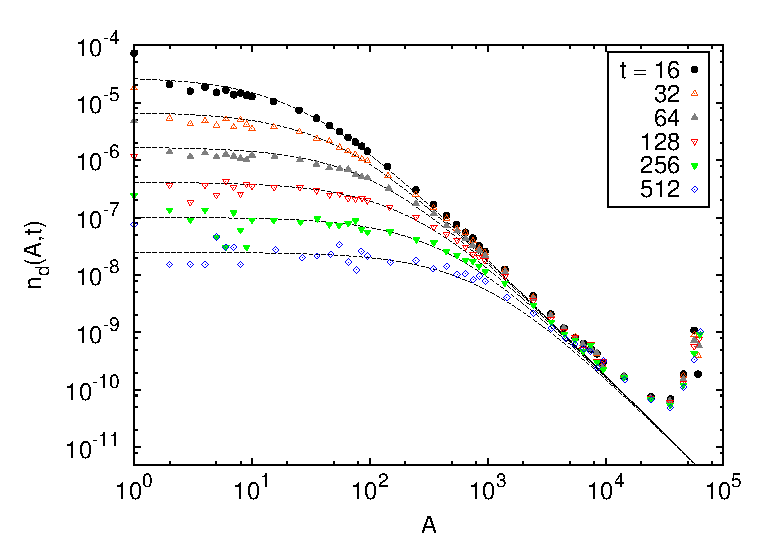
\includegraphics[width=14cm]{fig/areas_q2_L256_Tc_T0.eps}
 \caption{Distribuições das áreas dos domínios geométricos para $q=2$, em diferentes tempos, após um \textit{quench} de um estado de equilíbrio na temperatura inicial para $T_f=0$, para duas condições de temperatura inicial: no gráfico superior para $T_0 \rightarrow \infty$ e no inferior para $T_0 = T_c$. As linhas tracejadas correspondem a valores dados pelas Eq.~(\ref{eq.dq2tTinf}) e (\ref{eq.dq2tTc}), com $\lambda_d = 2.15$, enquanto os pontos resultam de simulações utilizando o método de Monte Carlo para uma rede quadrada com dimensão linear $L=256$, com uma média sobre 4000 amostras para cada caso. Os pontos que desviam das curvas, para áreas grandes, podem ser explicados pela existência de domínios percolantes, limitados pelas dimensões finitas da rede e computados com áreas menores do que teriam na ausência da limitação. Como o sistema é pequeno, vemos somente o início do comportamento do tipo lei de potência, esperado para grandes áreas.}
 \label{fig.areas_q2_L256}
\end{figure}


\section{Dinâmica para $q>2$}

Observa-se em sistemas com degenerescência múltipla no estado fundamental uma dinâmica de crescimento de domínios, após um \textit{quench} sobre a temperatura crítica, análoga à observada para sistemas com dupla degenerescência, conforme se pode observar na figura \ref{fig.PottsSnap}. Permanece válida a Eq.~(\ref{eq.AllenCahn}), sendo o parâmetro $\lambda$ dependente de $q$ e da temperatura.

\begin{figure}[h!]
 \setlength\fboxsep{0pt}
 \setlength\fboxrule{0.5pt}
 \centering
 \fbox{\includegraphics[width=35mm]{img/Potts_scr1.png}}
 \fbox{\includegraphics[width=35mm]{img/Potts_scr2.png}}
 \fbox{\includegraphics[width=35mm]{img/Potts_scr3.png}}
 \fbox{\includegraphics[width=35mm]{img/Potts_scr4.png}} \\
 (a) \hspace{30mm} (b) \hspace{30mm} (c) \hspace{30mm} (d) \vspace{3mm} \\
 \caption{Sequência mostrando a evolução de uma simulação de Monte Carlo do modelo de Potts com $q=3$, após um \textit{quench} da temperatura infinita para a temperatura zero. Os respectivos tempos são $t=2,8,32,256$ passos de Monte Carlo (MCs). Pontos pretos, brancos e vermelhos representam os diferentes estados possíveis para cada spin.}
 \label{fig.PottsSnap}
\end{figure}

Pode-se expressar a variação da área englobada por um \textit{hull} através de uma integral de caminho, sobre o \textit{hull}, da velocidade de um elemento diferencial do mesmo, de forma análoga ao que foi descrito para o caso com dupla degenerescência:
\begin{equation}
 \label{eq.DaDtq3}
 \frac{dA_h}{dt} = \oint v dl = -\frac{\lambda_h}{2\pi} \oint \kappa dl = -\lambda_h \left(1-\frac{1}{2\pi}\sum_i\alpha_i \right),
\end{equation}
onde a última igualdade é obtida a partir da forma geral do teorema de Gauss-Bonnet, e os $\alpha_i$ são os menores ângulos entre as retas tangentes às superfícies nos $n$ vértices ou junções triplas~\cite{LoureiroPRE}, conforme pode ser visto na figura~\ref{fig.GaussBonnet}. No caso $q=2$ não existem vértices, e a Eq.~(\ref{eq.DaDtq3}) se reduz à Eq.~(\ref{eq.DaDtq2}).

\begin{figure}
 \centering
 \includegraphics[width=70mm]{img/gauss_bonnet1.pdf}
 \includegraphics[width=70mm]{img/gauss_bonnet2.pdf} \\
 (a) \hspace{60mm} (b)
 \caption{Representação de vértices ou junções triplas. Em (a) temos o ângulo $\alpha_i$, que é o menor ângulo entre retas tangentes às interfaces entre domínios, no ponto $p$. Em (b) temos uma configuração análoga, no limite em que todos os ângulos entre domínios, nos pontos de junções triplas, são iguais a $2\pi/3$ ($\alpha_i = \pi/3$)~\cite{TeseMP}.}
 \label{fig.GaussBonnet}
\end{figure}

Para alguns sistemas, como modelos de espumas, os ângulos entre domínios, nos pontos de junções triplas, são todos iguais a $2\pi/3$. Restringindo a análise a sistemas desse tipo, ou que possam assim ser aproximados, e considerando uma correspondência de um para um entre vértices e lados, a Eq.~(\ref{eq.DaDtq3}) se reduz à lei de von Neumann~\cite{Neumann1952,Mullins1956} para a área $A_n$ de um \textit{hull} de $n$ lados:
\begin{equation}
 \label{eq.vonNeumann}
 \frac{dA_n}{dt} = \frac{\lambda}{6} \left( n-6 \right).
\end{equation}

Observando-se a Eq.~(\ref{eq.vonNeumann}), percebe-se que a evolução da área de um \textit{hull} depende fundamentalmente do número $n$ de lados do mesmo: para $n<6$ a área decresce, para $n>6$ ela cresce, e para $n=6$ se mantém constante. Domínios com poucos vizinhos tendem a diminuir e desaparecer, ao contrário dos com muitos vizinhos. Além disso, o número de lados de um \textit{hull} pode variar durante a evolução do sistema, à medida que seus domínios vizinhos evoluem ou desaparecem. Dessa forma, diferentemente do caso $q=2$, para $q>2$, em princípio não é possível obter uma expressão exata que determine a área de um \textit{hull} em um tempo $t$ qualquer, sendo conhecida sua área inicial~\cite{LoureiroPRE,LoureiroPRE2012}. No entanto, verifica-se que em determinados casos, como o do modelo com $q=3$, após um \textit{quench} a partir de um estado de equilíbrio em $T_0=T_c$, o sistema apresenta distribuições de \textit{hulls} e domínios geométricos com o mesmo comportamento observado para o caso $q=2$.

Na figura \ref{fig.AreasCol}, pode-se observar distribuições de áreas de domínios geométricos para $q=2$ e $q=3$, com $T_0 \rightarrow \infty$ e $T_0=T_c$, colapsadas para diversos tempos. O colapso obtido com o fator de escala $A \Rightarrow A/t$ era esperado, de acordo com a hipótese de escalamento dinâmico. Pode-se verificar que no caso $q=3$ com $T_0=T_c$, o colapso dos pontos se apresenta na forma esperada para uma dinâmica descrita pela Eq.~(\ref{eq.dq2tTc}), embora em princípio a mesma se aplique apenas ao caso $q=2$. A explicação definitiva para tal comportamento é ainda uma questão em aberto~\cite{LoureiroPRE}. Para o caso $q=3$ com $T_0 \rightarrow \infty$, a distribuição não apresenta cauda longa, não tendo uma forma compatível com a Eq.~(\ref{eq.dq2tTc}). Os dados utilizados na construção da figura \ref{fig.AreasCol} não incluem pontos associados com domínios percolantes, o que faz com que a distribuição não apresente picos para grandes tamanhos de domínios, como acontece na figura \ref{fig.areas_q2_L256}, mas apresente um desvio para baixo.

A temperatura final do \textit{quench} foi definida como $T_f=T_c/2$, em todos os casos. Assim evita-se o efeito de \textit{pinning}, que ocorre para $q > 2$, para temperaturas muito baixas, e que consiste no aparecimento de pontos ou regiões estáveis que interrompem a dinâmica~\cite{DerridaOliveiraStauffer}. Ao mesmo tempo, é suficientemente baixa para que permaneçam aplicáveis expressões que foram derivadas sem levar em consideração explicitamente a presença de flutuações térmicas.

\begin{figure}
 \centering
 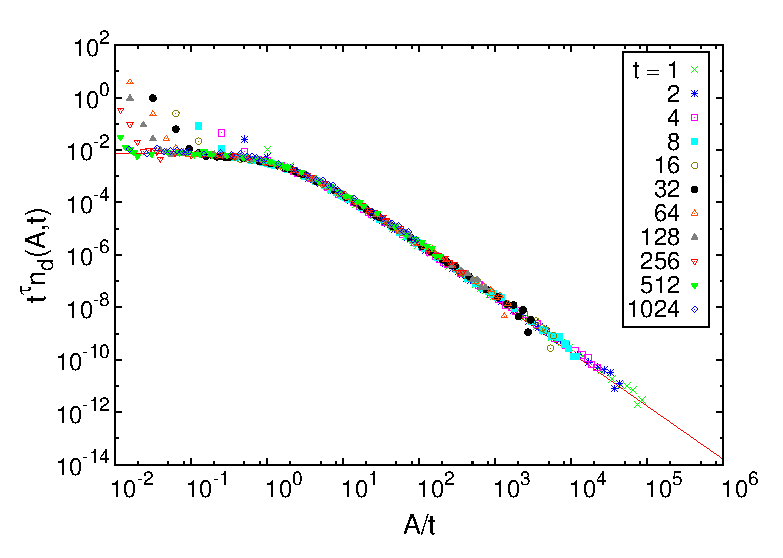
\includegraphics[width=7.65cm]{fig/areasnp_col_q2_L512_Tc_Tc2.eps}
 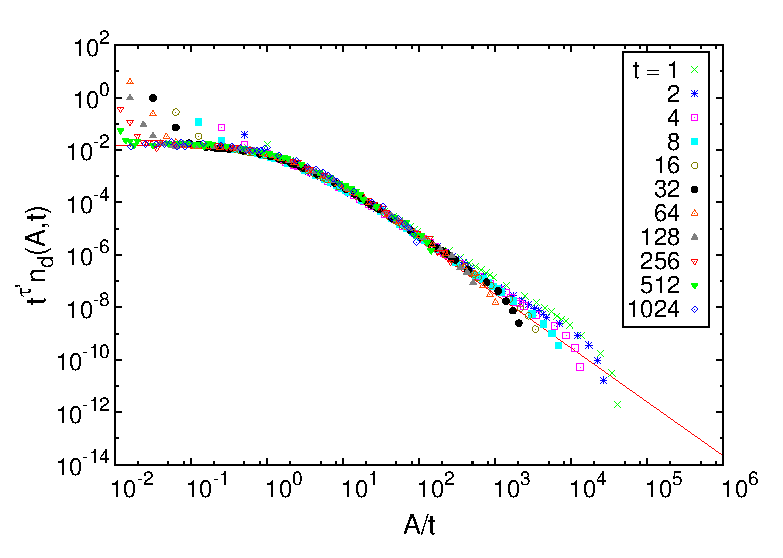
\includegraphics[width=7.65cm]{fig/areasnp_col_q2_L512_Tinf_Tc2.eps} \\
\hspace{8mm} (a) \hspace{70mm} (b)  \\
 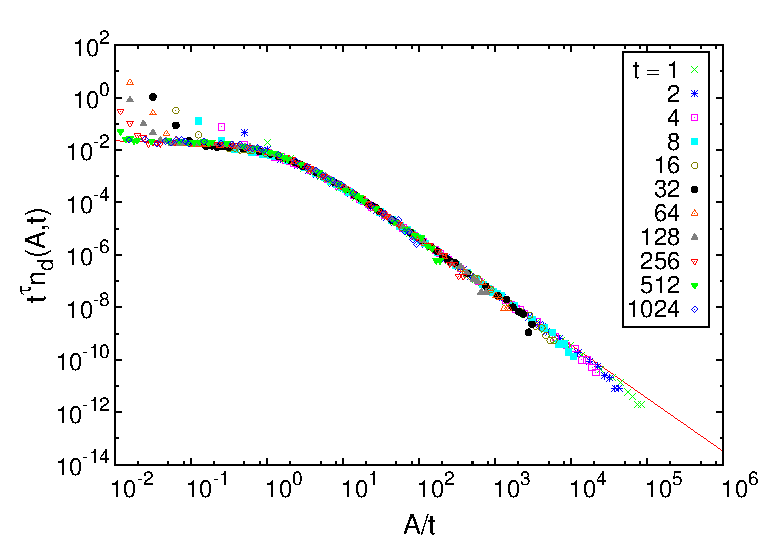
\includegraphics[width=7.65cm]{fig/areasnp_col_q3_L512_Tc_Tc2.eps}
 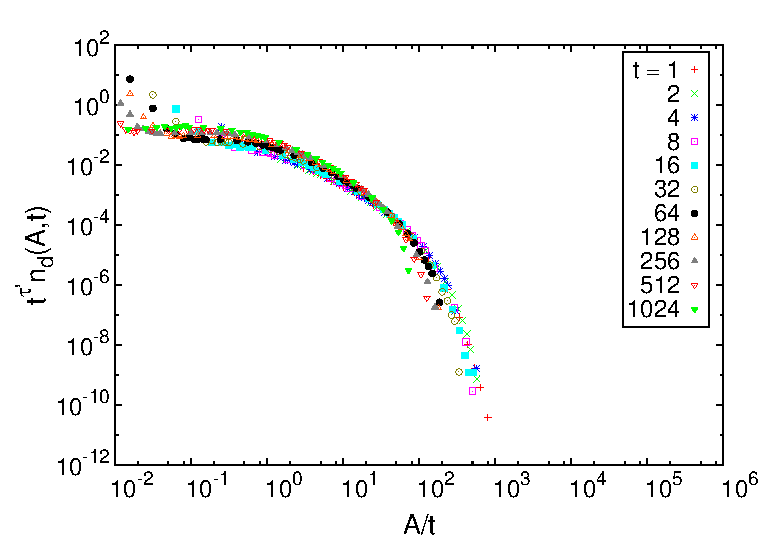
\includegraphics[width=7.65cm]{fig/areasnp_col_q3_L512_Tinf_Tc2.eps} \\
\hspace{8mm} (c) \hspace{70mm} (d)
 \caption{Distribuições das áreas dos domínios geométricos, colapsadas para diversos tempos. Em (a) e (b), para $q=2$ e em (c) e (d) para $q=3$. Em (a) e (c) o sistema sofreu um \textit{quench} a partir de um estado de equilíbrio em $T_0=T_c$ para $T_f=T_c/2$, enquanto que em (b) e (d) o \textit{quench} ocorreu de um estado de equilíbrio em $T_0 \rightarrow \infty$ para $T_f=T_c/2$. Os pontos resultam de simulações utilizando o método de Monte Carlo para uma rede quadrada com dimensão linear $L=512$, com uma média sobre 1000 amostras para cada caso. Os domínios percolantes não foram incluídos nas distribuições. As linhas sólidas correspondem a valores dados pelas Eq.~(\ref{eq.dq2tTinf}) e (\ref{eq.dq2tTc}), com mudanças nos parâmetros para o caso $q=3$.}
 \label{fig.AreasCol}
\end{figure}

